% =====================================================================
% Vibration-Consistency Training — SoICT 2026 submission (v3)
% Template: Springer CCIS / LNCS (llncs.cls)
%
% SoICT 2026: single-blind, 12 pages EXCLUDING references, Springer CCIS,
% PDF without page numbers, submitted via EasyChair.
%   abstract 09 Sep 2026 | full paper 16 Sep 2026
%   notification 12 Oct 2026 | camera-ready 23 Oct 2026
%
% EVERY NUMBER IN THIS PAPER COMES FROM A FILE IN THE REPOSITORY:
%   runs/paper_queue/UNIFIED.json   <- Tables 1, 2, 3, 4 (one eval code path,
%                                      3 seeds, mean +/- std)
%   runs/paper_queue/SUMMARY_DEPLOY.txt, RESULTS_FLIGHT_VAL.md <- Table 5
%   runs/paper_queue/BASELINES_TABLE.md <- params / GFLOPs
% See PAPER_INPUTS.md for the table -> file map.
% Anything marked \TODO{} is NOT measured yet. Do not submit with a \TODO.
% =====================================================================

\documentclass[runningheads]{llncs}

\usepackage{graphicx}
\usepackage{amsmath}
\usepackage{amssymb}
\usepackage{booktabs}
\usepackage{multirow}
\usepackage{xcolor}
\usepackage[hidelinks]{hyperref}

\newcommand{\TODO}[1]{\textcolor{red}{\textbf{[#1]}}}
\newcommand{\best}[1]{\textbf{#1}}
% mean +/- std gon trong bang: \ms{16.8}{0.7}
\newcommand{\ms}[2]{#1\,{\scriptsize$\pm$#2}}

\begin{document}

% ==================================================================
% Tieu de + tac gia + don vi   (file: sections/01_titlepage.tex)
% SoICT 2026 la SINGLE-BLIND -> GIU ten tac gia va affiliation.
% ==================================================================
\title{SteadyDet-N: A 4.6-GFLOP Person Detector That Leads Every
Compact Baseline Under UAV Vibration}

\titlerunning{SteadyDet-N: Compact Person Detection Under UAV Vibration}

\author{Nhan Le Thanh Huynh\inst{1} \and \TODO{Advisor Name}\inst{1}}

\authorrunning{N. L. T. Huynh et al.}

\institute{Ho Chi Minh City University of Technology and Education,
Ho Chi Minh City, Vietnam\\
\email{\TODO{your.email@hcmute.edu.vn}}}

\maketitle

% ==================================================================
% Abstract + keywords   (file: sections/02_abstract.tex)
% Doi khung 2026-07-26: phuong phap chinh = augmentation, consistency = ket qua am.
% Doi khung 2026-07-27a: them claim TRIEN KHAI (mCP).
% Doi khung 2026-07-27b: MODEL dung ten chinh. Abstract mo bang detector, va noi
%   ro "khong nua nao du mot minh" - do la lap luan giu cho kien truc la dong gop.
% ==================================================================
\begin{abstract}
We present SteadyDet-N, the nano variant of our SteadyDet family: a
$1.17$\,M-parameter, $4.6$-GFLOP anchor-free person
detector for multirotor UAVs, and show that it leads every compact baseline we
measured on the metric its deployment depends on, while losing to all of them on
the benchmark. That metric is accuracy under airframe vibration. Multirotors
vibrate whenever the rotors turn, and under a single evaluation protocol with
seeded corruption and error bars every compact detector we tested retains at most a
quarter of its clean average precision and is effectively blind at the moderate
severity of ordinary forward flight. The detector does not survive this by
architecture alone; untreated, it is the worst network in our table. What closes
the gap is deliberately plain. We replace half of each training batch with a copy
corrupted by a physically motivated model of motion blur, sensor noise and exposure
oscillation, and compute the ordinary detection loss on it. The corruption
preserves object coordinates so the labels stay valid, and it exists only during
training, so the deployed network is unchanged. Retention rises from
$16.8 \pm 0.7\%$ to $36.2 \pm 0.7\%$ and accuracy under moderate vibration by
$4.2\times$, at a cost of $9.7\%$ clean AP, enough to overtake all four YOLO nano
variants under vibration and a transformer of $28\times$ the size at the severity
of ordinary flight. Neither half suffices alone: the same regime applied to
YOLO11-n changes nothing, from scratch or from pretrained weights, and we rule out
pretraining, object scale and remaining headroom as explanations. Two further
controls make the result interpretable. Finetuning for the same $120$ epochs
without corruption leaves retention unchanged ($16.9 \pm 0.7\%$), and a consistency
formulation we expected to be stronger reaches only $30.0 \pm 0.6\%$ at $1.8\times$
the training cost. We report both negative results in full, since together they
identify what accuracy under vibration actually depends on.
\end{abstract}

\keywords{Tiny object detection \and Robustness \and Data augmentation \and UAV
\and Edge deployment.}


% ==================================================================
% 1. Introduction   (file: sections/03_introduction.tex)
% ==================================================================
\section{Introduction}
\label{sec:intro}

\begin{figure}[t]
\centering
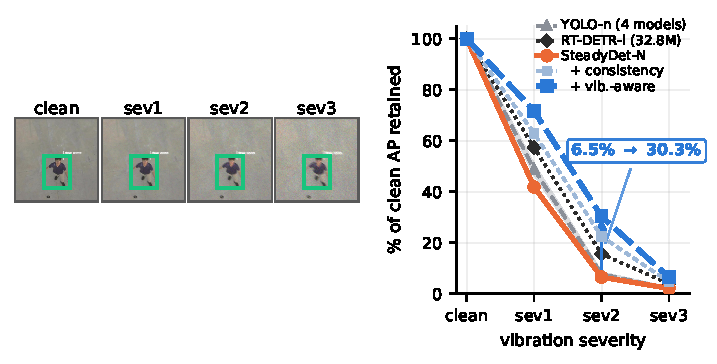
\includegraphics[width=0.95\textwidth]{figures/fig1_teaser.pdf}
\caption{\textbf{Compact aerial detectors go blind when the airframe vibrates.}
A flight frame under each VisDrone-Shake severity (sev1 and sev2 are ordinary flight,
not a fault), and the fraction of clean AP that survives on VisDrone-person, over
three seeds. Every published detector collapses at the same rate: the failure
belongs to the regime, not to one network.}
\label{fig:teaser}
\end{figure}

A detector that scores well on an aerial benchmark can still be unusable on an
actual aircraft, for a physical reason the literature largely ignores: a
multirotor vibrates. Rotor imbalance, motor harmonics and frame resonance
transmit high-frequency motion to the camera, and because the sensor integrates
over a finite exposure, that motion appears as directional blur, elevated noise
and frame-to-frame brightness oscillation. Unlike weather or occlusion this
corruption is not occasional; it is present whenever the rotors are spinning.

We began by measuring how much it matters, on our own detector first. SteadyDet-N
is an anchor-free network of $1.17$\,M parameters and $4.6$ GFLOPs built for
tiny-person detection from a UAV, and under a four-level vibration model it falls
from $0.189$ to $0.012$ average precision at moderate severity, retaining
$16.8 \pm 0.7\%$ of its clean accuracy. Fig.~\ref{fig:teaser} shows the collapse is
not ours alone: every published detector we measured falls at the same rate. A
detector blind whenever the aircraft is airborne is not a detector, and on this
axis the entire compact-detection literature is in the same position.

The obvious responses are unattractive on a small UAV. Isolation and gimbals cost
mass, payload and power; deblurring adds a second network to a pipeline that must
already fit a detector, a tracker and a controller into a $50$\,ms budget on a
passively cooled board. Every one pays at run time, on the platform least able to
afford it.

The response we test is deliberately blunt: put the vibration into the training
distribution. Each batch is replaced, with probability one half, by a corrupted copy
drawn from a physically motivated model of rotor-induced degradation, and the
ordinary detection loss is computed on whatever the network receives. Because blur,
noise and brightness scaling do not move objects, the labels remain valid and
nothing else changes. At inference the corruption does not exist and the exported
network is identical to the baseline, so the robustness costs nothing where cost is
felt.

Neither the network nor the regime suffices alone, and we show this rather than
assert it. Untreated, SteadyDet-N is the least accurate row in our table under
vibration; applied to YOLO11-n, the identical regime changes nothing at all, from
COCO weights or from scratch. Only the combination moves, and it moves past all
four YOLO nano variants while remaining the smallest and cheapest network compared.
That null result is also what keeps the comparison fair: our treated detector is
measured against a baseline that cannot be improved the same way, not against a
handicapped one.

We also tried something more elaborate, a consistency formulation, and report that
it is measurably worse at $1.8\times$ the training cost. A control contradicting the
authors' expectation is worth more to a reader than one confirming it.

Our contributions are: \textbf{(i)} \emph{SteadyDet-N with its training regime},
which at $1.17$\,M parameters and $4.6$ GFLOPs loses to every YOLO nano variant on
clean VisDrone and leads all of them on accuracy under vibration, exceeding
RT-DETR-l at $28\times$ its size at the severity of ordinary forward flight
(Section~\ref{sec:baselines}); \textbf{(ii)} \emph{VisDrone-Shake}, a seeded
four-level vibration protocol under which every detector we tested loses
$74$ to $83\%$ of its average precision (Sections~\ref{sec:shake}
and~\ref{sec:baselines}); \textbf{(iii)} \emph{vibration-aware training}, raising
retention from $16.8 \pm 0.7\%$ to $36.2 \pm 0.7\%$ at zero inference cost, with
the control showing the $120$ additional epochs contribute nothing on their own
($16.9 \pm 0.7\%$) (Section~\ref{sec:mainresults}); \textbf{(iv)} a controlled
negative result, that the consistency formulation we expected to be better is
measurably worse while costing more to train (Section~\ref{sec:mainresults}); and
\textbf{(v)} evidence that the architecture and the regime are each necessary,
since the same regime applied to YOLO11-n produces no effect at all and three
candidate explanations for that are tested and rejected
(Section~\ref{sec:generality}).

% ==================================================================
% 2. Related Work   (file: sections/04_related_work.tex)
% ==================================================================
\section{Related Work}
\label{sec:related}

\subsubsection{Robustness to corruption.}
ImageNet-C~\cite{hendrycks2019benchmarking} established the mean corruption
protocol we adapt, later extended to detection~\cite{michaelis2019benchmarking}.
Those benchmarks sample a broad corruption taxonomy suited to general vision; on a
multirotor the distribution is concentrated instead, set by rotor dynamics and
exposure time, so we build a domain-specific protocol rather than reuse a generic
one. Motion deblurring~\cite{nah2017deepdeblur} attacks the same degradation by
restoring the image, adding a second network to the critical path; we leave the
inference graph untouched.

\subsubsection{Consistency regularisation.}
Agreement between perturbed views underpins semi-supervised
learning~\cite{sajjadi2016regularization,tarvainen2017mean,sohn2020fixmatch} and
self-supervised representation learning~\cite{chen2020simclr,grill2020byol}. Our
use differs in purpose: the data are fully labelled, so the term is not a substitute
for supervision but a directed statement about which nuisance to discard. The
closest supervised analogue is consistency-based domain
adaptation~\cite{french2018selfensembling}, where the perturbation models a domain
gap rather than a sensing process.

\subsubsection{Efficient aerial detection.}
VisDrone~\cite{zhu2021visdrone} is dominated by instances below $32\times32$ pixels,
in the tiny-object regime of~\cite{yu2020tinyperson,cheng2023sod}. Efficient
detectors here combine depthwise-separable
backbones~\cite{qin2024mnv4,sandler2018mobilenetv2}, cross-stage partial
connections~\cite{wang2020cspnet}, feature pyramids~\cite{tan2020efficientdet} and
anchor-free heads~\cite{ge2021yolox}, with RemDet~\cite{chen2025remdet} targeting
small-object downsampling and recent YOLO generations moving to NMS-free
prediction~\cite{wang2024yolov10}; IoU losses are unstable for tiny boxes,
motivating NWD~\cite{wang2021nwd} blended with CIoU~\cite{zheng2020diou} alongside
\cite{li2020gfl} and~\cite{feng2021tood}. All of it optimises clean accuracy per
unit of compute. We take a detector from this family and ask a different question:
how much of that accuracy survives the aircraft it is meant to fly on.


\section{Method}
\label{sec:method}
% ==================================================================
% 3.1 Detector platform.
% Hinh fig3_arch GANH phan mo ta kien truc -> van o day co y giu NGAN:
% chi noi cai gi hinh khong noi duoc (ly do thiet ke + con so chi phi).
% Kien truc KHONG phai dong gop cua bai (Section 4.4 noi thang the).
% file: sections/05_platform.tex
% ==================================================================
\subsection{Detector Platform}
\label{sec:platform}

\begin{figure}[t]
\centering
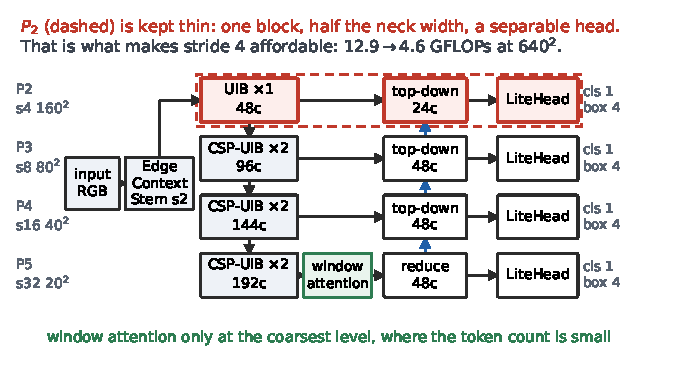
\includegraphics[width=0.95\textwidth]{figures/fig3_arch.pdf}
\caption{SteadyDet-N; resolution decreases down the page. Compute is deliberately
asymmetric: the stride-4 row $P_2$ (dashed), where most drone-scale persons are
resolved, carries one block, a half-width neck branch and a separable head, while
the two-block CSP stages and the attention sit where the maps are small. Blue
arrows are the top-down upsample-and-fuse path. That is what keeps $P_2$ at $4.6$
instead of $12.9$ GFLOPs.}
\label{fig:arch}
\end{figure}

SteadyDet-N is an anchor-free single-stage detector of $1.17$\,M parameters and
$4.6$ GFLOPs at $640\times640$ (Fig.~\ref{fig:arch}). We are explicit about what we
do and do not claim for it. It does not lead its class in clean accuracy and
Section~\ref{sec:baselines} reports that plainly; what we claim is its accuracy
under vibration once the corruption is in its training distribution, a combination
no baseline we measured matches. The design choice that matters most for this is
that it keeps a stride-4 level, since at the altitudes VisDrone covers a person
occupies fewer than $32\times32$ pixels and detectors beginning at stride 8 discard
that signal before detection begins.

Keeping stride 4 is what makes such a detector expensive. At $640\times640$ the $P_2$
map is $160\times160$, so every operation there costs $16\times$ what it costs at
$P_3$, and in an earlier configuration of ours the $P_2$ head alone consumed $1.82$
GMACs, $28\%$ of total compute. Fig.~\ref{fig:arch} shows the three changes that cut
the total to $4.6$ GFLOPs without giving up stride 4: one Universal Inverted
Bottleneck~\cite{qin2024mnv4} block at $P_2$ instead of three, windowed
self-attention~\cite{liu2021swin} at $P_5$ only, and a depthwise-separable head in
place of a five-convolution decoupled one. Deeper stages use cross-stage partial
blocks~\cite{wang2020cspnet}.

Regression blends the Normalized Wasserstein Distance~\cite{wang2021nwd} with
CIoU~\cite{zheng2020diou} by ground-truth area, since IoU gradients are unstable for
tiny boxes; classification uses~\cite{li2020gfl} and assignment
follows~\cite{feng2021tood}, modified so each small ground truth gets several
positives. Optimisation blends Muon~\cite{jordan2024muon} and SGD.

% ==================================================================
% 3.2 Giao thuc VisDrone-Shake   (file: sections/06_shake_protocol.tex)
% ==================================================================
\subsection{The VisDrone-Shake Protocol}
\label{sec:shake}

Measuring vibration robustness needs a corruption model reflecting rotorcraft
physics rather than a generic suite. Three effects dominate. \textbf{Directional
motion blur}: camera displacement during exposure integrates the scene along the
motion direction, modelled as convolution with a linear kernel. \textbf{Sensor
noise}: blur reduces effective signal and automatic exposure compensates by raising
gain, amplifying read noise. \textbf{Exposure oscillation}: rotor frequency beating
against the rolling shutter gives frame-to-frame brightness fluctuation, applied
multiplicatively.

The three are composed at three severity levels above clean, parameterised by (blur
kernel length in pixels, noise $\sigma$, brightness range) as
sev1 $=(5,\,0.02,\,{\pm}10\%)$, sev2 $=(9,\,0.04,\,{\pm}20\%)$ and
sev3 $=(15,\,0.06,\,{\pm}30\%)$, with blur orientation drawn uniformly per batch.
Levels sev1 and sev2 correspond to a well-balanced airframe in steady flight; sev3 to
severe excitation such as an unbalanced rotor. None of the three translates objects, so
ground-truth boxes stay valid and the same operator serves as both a training
perturbation and a fixed evaluation protocol.

Following~\cite{hendrycks2019benchmarking} we report the mean corrupted precision
$\mathrm{mCP}$ over the three corrupted levels and the retention ratio
$\mathrm{retain}\% = 100 \cdot \mathrm{mCP}/\mathrm{AP}_{\mathrm{clean}}$, which
measures how much of a detector's accuracy survives flight rather than how accurate
it is on the ground. Two detectors with equal clean AP can differ widely in it.

\subsubsection{The protocol is stochastic, so it must be seeded.}
Blur orientation, noise and brightness are drawn at random, so a single pass is one
draw rather than a measurement: unseeded, retention for one checkpoint varied by
more than a point between passes, enough to manufacture a modest improvement. We
reseed before every severity pass and report mean and standard deviation over three
seeds. Gains smaller than a benchmark's own run-to-run spread are not gains.

% ==================================================================
% 3.3 Vibration-Aware Training  <-- DONG GOP CHINH (doi khung 2026-07-26)
%
% LICH SU: ban truoc trinh bay CONSISTENCY la phuong phap chinh. Doi chung
% augment-only (Section 4.2) cho thay augmentation THANG consistency 36.2 vs
% 30.0 retain, nen phuong phap chinh doi thanh augmentation, con consistency
% tro thanh BIEN THE duoc bao cao kem ket qua am. Xem paper/PENDING_ABLATION.md.
% file: sections/07_vibcon.tex
% ==================================================================
\subsection{Vibration-Aware Training}
\label{sec:vibcon}

\begin{figure}[t]
\centering
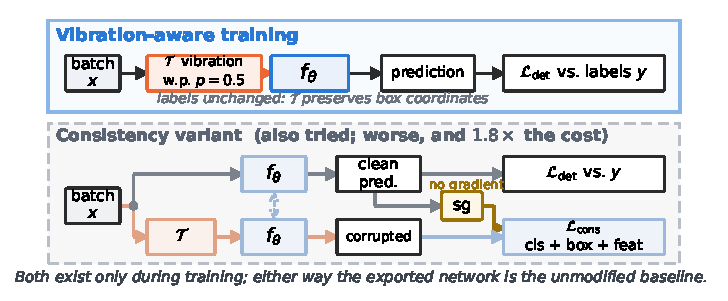
\includegraphics[width=0.95\textwidth]{figures/fig2_method.pdf}
\caption{Vibration-aware training (top) and the consistency variant we also tried
(bottom). The method we recommend is the simple one: corrupt a fraction of each
batch with $\mathcal{T}$ and compute the ordinary detection loss on the corrupted
image. The variant forwards the batch twice and adds a consistency term against a
stop-gradient copy of the clean prediction. Neither survives into deployment: the
exported network is unchanged in either case.}
\label{fig:method}
\end{figure}

Let $\mathcal{T}$ denote the stochastic vibration operator of
Section~\ref{sec:shake}, with severity and blur orientation resampled per batch.
Fig.~\ref{fig:method} contrasts the method with the variant of
Section~\ref{sec:mainresults}; the method is one line. During training, each batch $x$ is replaced by
$\mathcal{T}(x)$ with probability $p = 0.5$, and the ordinary detection loss is
computed on whatever image the network receives:
\begin{equation}
\mathcal{L} = \mathcal{L}_{\det}\bigl(f_\theta(\hat{x}), y\bigr),
\qquad
\hat{x} = \begin{cases}
\mathcal{T}(x) & \text{with probability } p,\\
x & \text{otherwise.}
\end{cases}
\label{eq:vibaware}
\end{equation}
Because $\mathcal{T}$ preserves object coordinates the labels $y$ need no
adjustment, which is what makes the substitution legitimate at all. No module is
added, no second forward pass is required, and the exported graph is structurally
identical to the baseline, so inference cost is unchanged. The only training cost
is the corruption operator, a depthwise convolution and two elementwise
operations.

\subsubsection{Why this is not simply data augmentation as usually understood.}
Standard detection augmentation samples nuisances the training distribution already
contains: flips, scale jitter, colour shifts. $\mathcal{T}$ samples one it does
\emph{not}, because VisDrone is collected from stable platforms. This is therefore
not a regularisation trick but a correction of a mismatch between the data a
detector is trained on and the conditions it will meet, which is why the severities
in Section~\ref{sec:shake} are chosen to bracket rotorcraft flight rather than to
maximise validation score.

\subsubsection{A consistency variant, which we report because it is worse.}
Before running the control, we expected that a stronger signal could be extracted
from the corrupted view than the detection loss provides. The variant forwards both
$x$ and $\mathcal{T}(x)$ through the same weights, computes the detection loss on
the clean branch only, and adds a consistency term that pulls the corrupted
prediction towards a stop-gradient copy of the clean one,
\begin{equation}
\mathcal{L} = \mathcal{L}_{\det}\bigl(f_\theta(x), y\bigr)
 + \lambda_{\mathrm{vib}} \, \mathcal{L}_{\mathrm{cons}}
 \bigl(f_\theta(\tilde{x}),\; \mathrm{sg}[f_\theta(x)]\bigr),
\qquad \lambda_{\mathrm{vib}} = 0.5,
\label{eq:vibcon}
\end{equation}
where $\mathcal{L}_{\mathrm{cons}}$ sums, over pyramid levels, a temperature-scaled
cross-entropy on objectness, a smooth $L_1$ term on boxes gated by clean-branch
objectness, and a squared error between neck features. Exact forms are in the
released code. The stop-gradient is not optional: without it the objective is
minimised by degrading the clean prediction towards the corrupted one, lowering the
loss while destroying the detector. The reasoning was that the clean prediction
says more than the hard label, and that blur destroys exactly that structure.
Section~\ref{sec:mainresults} shows it does not survive measurement.

\subsubsection{Training procedure.}
We apply the corruption as a finetuning stage rather than from scratch: starting
from a converged baseline checkpoint, we finetune for $120$ epochs at batch size
$8$ with gradient accumulation $12$, MuSGD at learning rate $2\times10^{-3}$, and a
three-epoch warm-up before the corruption is switched on. The method can therefore
be applied to a detector that has already been trained, without repeating its
schedule. Checkpoints are selected by clean validation AP, the same rule used for
the baseline, so no checkpoint in this paper is chosen using the robustness
protocol it is evaluated on.


\section{Experiments}
\label{sec:exp}
% ==================================================================
% 4.1 Setup thi nghiem   (file: sections/08_exp_setup.tex)
% ==================================================================
\subsection{Setup}
\label{sec:setup}

We evaluate on the person categories of VisDrone-DET~\cite{zhu2021visdrone}, merging
\texttt{pedestrian} and \texttt{people} into one class, which matches a following system
that must track any human regardless of pose: $6471$ training and $548$ validation
images.

\subsubsection{One evaluation code path for every model.}
Each detector family ships its own harness with its own confidence threshold,
detection cap and area convention, and differences of several AP points can be
produced by the harness alone. We therefore evaluate \emph{every} model in
\emph{every} table below with one script: images are letterboxed to $640\times640$ by the same loader, predictions are
thresholded at confidence $0.01$, reduced by NMS at IoU $0.5$, capped at $300$
detections per image, and scored by \texttt{pycocotools} on identically constructed
ground truth. Baselines receive the same pre-processed tensors as ours, so no model
sees a different image. Every corrupted evaluation is repeated with three seeds
($0,1,2$), reseeding the corruption sampler before each severity pass, and reported as
mean $\pm$ sample standard deviation; clean evaluation is deterministic.

\subsubsection{Training.}
Training uses only VisDrone, with no COCO person data, so comparison against prior
work is not confounded by extra training data. Baselines start from COCO-pretrained
weights and ours from scratch, which favours them, and each family uses its own
recommended optimiser and schedule rather than a shared one, since a shared one
destroys some of them: under default CNN optimiser selection RT-DETR diverges by
epoch four. All models train on a single RTX~4060 Laptop GPU (8\,GB), one run per
configuration.

% ==================================================================
% 4.2 Ket qua chinh + 2 doi chung + generality.
% So lieu: runs/paper_queue/UNIFIED.json (sinh dong bang bang paper/make_tables.py)
% file: sections/09_exp_main.tex
% ==================================================================
\subsection{Main Results}
\label{sec:mainresults}

\begin{table}[t]
\centering
\caption{VisDrone person subset, $640\times640$, \texttt{pycocotools}. Clean
accuracy is deterministic; corrupted columns are mean $\pm$ std over three seeds.
Within each block the rows differ in exactly one variable and share the schedule,
learning rate and augmentation pipeline. Reading the SteadyDet-N block downwards
identifies where the robustness comes from: not from the extra epochs, and not
from the consistency term. The YOLO11-n block, added as a test of generality,
shows the regime having no effect at all outside our detector family.}
\label{tab:main}
\setlength{\tabcolsep}{3.4pt}
\begin{tabular}{lccc|cccc}
\toprule
 & \multicolumn{3}{c|}{clean} & \multicolumn{4}{c}{under vibration (AP$_{50:95}$)} \\
Model & AP$_{50:95}$ & AP$_{50}$ & AP$_{75}$ & sev1 & sev2 & sev3 & retain\% \\
\midrule
\multicolumn{8}{l}{\emph{SteadyDet-N (1.17\,M, 4.6 GFLOPs)}} \\
\quad baseline             & 0.1892 & 0.5127 & 0.0811
    & \ms{0.0792}{.0026} & \ms{0.0123}{.0013} & \ms{0.0040}{.0005} & \ms{16.8}{.7} \\
\quad + 120 ep, no vibration & 0.1823 & 0.4984 & 0.0762
    & \ms{0.0761}{.0028} & \ms{0.0125}{.0005} & \ms{0.0040}{.0005} & \ms{16.9}{.7} \\
\quad + consistency variant & 0.1746 & 0.4837 & 0.0728
    & \ms{0.1098}{.0010} & \ms{0.0392}{.0021} & \ms{0.0081}{.0011} & \ms{30.0}{.6} \\
\quad \textbf{+ vibration-aware} & 0.1708 & 0.4731 & 0.0715
    & \best{\ms{0.1223}{.0014}} & \best{\ms{0.0518}{.0019}} & \best{\ms{0.0111}{.0002}} & \best{\ms{36.2}{.7}} \\
\midrule
\multicolumn{8}{l}{\emph{SteadyDet-W (1.00\,M, 12.9 GFLOPs)}} \\
\quad baseline           & 0.2349 & 0.5800 & 0.1305
                 & \ms{0.1260}{.0023} & \ms{0.0258}{.0022} & \ms{0.0046}{.0026} & \ms{22.2}{.9} \\
\quad + consistency variant & 0.2207 & 0.5561 & 0.1202
                 & \ms{0.1309}{.0026} & \ms{0.0580}{.0007} & \ms{0.0132}{.0016} & \ms{30.5}{.6} \\
\quad \textbf{+ vibration-aware} & 0.2219 & 0.5511 & 0.1279
                 & \best{\ms{0.1583}{.0013}} & \best{\ms{0.0839}{.0001}} & \best{\ms{0.0200}{.0012}} & \best{\ms{39.4}{.3}} \\
\midrule
\multicolumn{8}{l}{\emph{YOLO11-n, trained from scratch on the same data (2.59\,M, 6.4 GFLOPs)}} \\
\quad baseline           & 0.2588 & 0.5842 & 0.1839
                 & \ms{0.1398}{.0057} & \ms{0.0248}{.0022} & \ms{0.0052}{.0021} & \ms{21.9}{1.1} \\
\quad + 120 ep, no vibration & 0.2641 & 0.5897 & 0.1857
                 & \ms{0.1410}{.0036} & \ms{0.0226}{.0026} & \ms{0.0062}{.0030} & \ms{21.4}{.9} \\
\quad + vibration-aware  & 0.2579 & 0.5835 & 0.1806
                 & \ms{0.1384}{.0037} & \ms{0.0227}{.0017} & \ms{0.0055}{.0026} & \ms{21.5}{.8} \\
\bottomrule
\end{tabular}
\end{table}

Table~\ref{tab:main} reports the primary results. On SteadyDet-N the baseline
retains $16.8 \pm 0.7\%$ of its clean accuracy under vibration; training with the
corruption raises this to $36.2 \pm 0.7\%$, a factor of $2.15$. At sev2, the
moderate vibration of an airframe in forward flight, the baseline retains $6.5\%$
of its clean accuracy and is effectively blind, while the vibration-aware model
retains $30.3\%$ and is $4.2\times$ better in absolute AP, while clean AP falls by
$9.7\%$. For an airborne system that exchange is favourable: a detector a tenth
less accurate on the ground and four times more accurate with the rotors running is
the more useful one. The two middle rows are what make the result interpretable,
and each was run because a reader would otherwise be entitled to doubt the first.

\subsubsection{The gain is not an artefact of the extra epochs.}
The regime is applied as a finetuning stage, so the vibration-aware model has seen
$120$ epochs that the baseline has not. Finetuning the baseline for the same $120$
epochs with the corruption switched off leaves retention at $16.9 \pm 0.7\%$
against the baseline's $16.8 \pm 0.7\%$, a difference well inside one standard
deviation. Continued training contributes nothing. Clean accuracy does drift down
over those epochs ($0.1892$ to $0.1823$), so roughly a third of the clean-AP cost
of the vibration-aware model is the finetuning rather than the corruption.

\subsubsection{The consistency term does not help; it hurts.}
We expected the opposite. The variant of Eq.~\ref{eq:vibcon} reaches
$30.0 \pm 0.6\%$, $6.2$ points below the simple substitution and roughly nine times
the seed-to-seed spread of either measurement, so the ordering is not noise. It is
worse in absolute terms at every severity, not only after normalisation, and costs
$1.8\times$ the training time. Our reading is that the consistency term, computing
the detection loss on the clean branch only, never asks the network to \emph{detect}
under blur; it asks only that its corrupted predictions resemble its clean ones, a
weaker requirement that can be satisfied by making both less committed. The simple
substitution puts the corrupted image directly against the labels. We offer this as
an explanation rather than a demonstration.

\subsubsection{Generality, and where it stops.}
\label{sec:generality}
A regime that works on exactly one architecture is hard to distinguish from a
fortunate interaction with it. This one carries across both of our detectors and
then stops, and the stop is worth as much detail as the success. The middle block
of Table~\ref{tab:main} repeats the experiment on SteadyDet-W, an earlier detector
of ours with a full-width stride-4 branch and non-separable five-convolution heads,
so that despite slightly \emph{fewer} parameters ($1.00$ against $1.17$\,M) it
costs $2.8\times$ the compute and is the stronger on clean data. Nothing was
retuned. Retention rises from $22.2 \pm 0.9\%$ to
$39.4 \pm 0.3\%$, a gain of $17.2$ points against $19.3$, and the consistency
variant again falls short at $30.5 \pm 0.6\%$. Direction, magnitude and the
ordering of the two variants all reproduce on a network of different width, depth
and head design.

The lower block applies the identical regime to YOLO11-n, and nothing happens:
$21.9 \pm 1.1\%$ becomes $21.5 \pm 0.8\%$, with the no-vibration control at
$21.4 \pm 0.9\%$. The consistency variant on the COCO-pretrained checkpoint
likewise moved $20.1 \pm 1.2\%$ to $19.2 \pm 1.3\%$. Logging the corrupted-batch
substitution during training confirms the treatment was applied and not silently
skipped. We tested three explanations and none survived.

\emph{Pretraining.} If the baseline already holds blur-tolerant features there is
nothing left to teach. Retraining YOLO11-n from random initialisation leaves the
regime at $-0.3$ points, exactly as from pretrained weights, and the pretrained
checkpoint is the \emph{less} robust of the two ($20.1$ against $21.9\%$).

\emph{Object scale.} Our detectors carry a stride-4 level and YOLO11-n starts at
stride~8, so perhaps only the finest level has anything to gain. Broken out on
small objects the gain is $+18.7$ points against $+19.3$ overall, tracking the
aggregate rather than concentrating in it, and nearly every instance in this subset
is small for both families (AP$_s$ $0.2741$ of AP $0.2768$ for YOLO11-n). There is
no scale split available to carry the argument.

\emph{Headroom.} SteadyDet-W starts at $22.2 \pm 0.9\%$ and YOLO11-n from scratch at
$21.9 \pm 1.1\%$, the same point within noise. One gains $17.2$ points and the
other none.

What remains is the architecture or the loss, which our detectors share and
YOLO11-n does not: a stride-4 branch, a normalised-Wasserstein and CIoU box
objective, quality focal classification, and direct rather than distributional box
regression. One non-responding model cannot separate these, so we state the claim
at the scope the evidence supports. Vibration-aware training is a large,
reproducible gain for the detector family of Section~\ref{sec:platform} and does
nothing on the one outside architecture we tried; locating the boundary is the most
useful experiment this work leaves open.

% 4.3 Generality DA GOP vao 09_exp_main.tex (chung Table 1, truoc do lap y).
% File 10_exp_generality.tex con trong repo neu muon tach lai.
% % ==================================================================
% 4.3 Tinh tong quat tren kien truc khac (v15)
% KHONG co bang rieng — dung LAI khoi v15 trong Table~\ref{tab:main}.
% file: sections/10_exp_generality.tex
% ==================================================================
\subsection{Generality Across Architectures}
\label{sec:generality}

A regulariser that works on exactly one architecture is hard to distinguish from a
fortunate interaction with it. The lower block of Table~\ref{tab:main} therefore
repeats the experiment on SteadyDet-W, an earlier detector of ours with a full-width
stride-4 branch and non-separable five-convolution heads, so that although it has
slightly \emph{fewer} parameters ($1.00$ against $1.17$\,M) it costs $2.8\times$ the
compute and is the stronger of the two on clean data. Nothing was retuned.

The outcome reproduces: retention rises from $22.2 \pm 0.9\%$ to $30.5 \pm 0.6\%$,
accuracy at sev2 improves $2.25\times$, and clean AP falls by $6.0\%$. The two arrows
in Fig.~\ref{fig:tradeoff} are the same shape, which is the point: the mechanism acts
on the training objective rather than on a particular inductive bias. The magnitude is
smaller than on SteadyDet-N ($+8.3$ against $+13.2$ points), consistent with
SteadyDet-W starting from a higher baseline retention.

\subsubsection{A note on checkpoint selection.}
The final checkpoint of this run reaches a higher retention than the one we
report, $33.4 \pm 0.3\%$ against $30.5 \pm 0.6\%$. We report the lower figure
because it comes from the checkpoint selected by clean validation AP, which is the
rule applied to the baseline; taking the final checkpoint for our model while
taking the best-validation checkpoint for the baseline would be two rules, and the
difference between them here is $2.9$ points, a third of the effect we are
claiming. We state the rule and accept the number it produces.

\subsubsection{Scope of this evidence.}
Both architectures are ours and share the loss function, assignment strategy and
optimiser, so this shows insensitivity to backbone design rather than independence
from our whole training recipe. We prefer to state that limit than to describe two
detectors of our own as an architecture-agnostic result; the experiment that would
settle it is in Section~\ref{sec:limitations}.

% ==================================================================
% 4.4 So sanh voi detector nhe (MOT giao thuc duy nhat)
% file: sections/11_exp_baselines.tex
% So lieu: runs/paper_queue/UNIFIED.json (accuracy + mCP + retain)
%          runs/paper_queue/BASELINES_TABLE.md (params / GFLOPs)
% ==================================================================
\subsection{Comparison with Lightweight Detectors}
\label{sec:baselines}

Table~\ref{tab:baselines} compares five detectors spanning three paradigms against
ours. Every row, including the corrupted columns, came from the single evaluation
path of Section~\ref{sec:setup}. We report it in full rather than selectively, and
the two accuracy columns disagree about who wins.

\begin{table}[t]
\centering
\caption{VisDrone person subset, every row measured by the same evaluation code
(Section~\ref{sec:setup}). $\mathrm{mCP}$ is mean AP$_{50:95}$ over the three
vibration levels, that is, accuracy \emph{in flight}; retention is
$\mathrm{mCP}/\mathrm{AP}_{\mathrm{clean}}$, mean $\pm$ std over three seeds. YOLO
and RT-DETR rows start from COCO-pretrained weights while SteadyDet rows train from
scratch, which favours the baselines. \emph{The clean and the mCP columns rank the
table differently, and mCP is the one the aircraft experiences.}}
\label{tab:baselines}
\setlength{\tabcolsep}{4.5pt}
\begin{tabular}{lcccccc}
\toprule
Model & Params (M) & GFLOPs & AP$_{50}$ & AP$_{50:95}$ & mCP & retain\% \\
\midrule
RT-DETR-l                   & 32.81 & 108.0 & 0.5909 & 0.2502$^\dagger$ & 0.0641 & \ms{25.6}{1.1} \\
YOLOv10-n                   & 2.71 & 8.4 & 0.6043 & 0.2730 & 0.0538 & \ms{19.7}{1.4} \\
YOLOv8-n                    & 3.01 & 8.2 & 0.6033 & 0.2684 & 0.0522 & \ms{19.5}{.8} \\
YOLO26-n                    & 2.50 & 5.8 & 0.5898 & 0.2675 & 0.0507 & \ms{19.0}{1.0} \\
YOLO11-n                    & 2.59 & 6.4 & \best{0.6119} & \best{0.2768} & 0.0557 & \ms{20.1}{1.2} \\
\quad + vib.-aware          & 2.59 & 6.4 & 0.6057 & 0.2700 & 0.0542 & \ms{20.1}{1.3} \\
\midrule
SteadyDet-W                  & 1.00 & 12.9 & 0.5800 & 0.2349 & 0.0521 & \ms{22.2}{.9} \\
\quad \textbf{+ vib.-aware} & 1.00 & 12.9 & 0.5511 & 0.2219 & \best{0.0874} & \best{\ms{39.4}{.3}} \\
SteadyDet-N                  & \textbf{1.17} & \textbf{4.6} & 0.5127 & 0.1892 & 0.0318 & \ms{16.8}{.7} \\
\quad + consistency         & 1.17 & 4.6 & 0.4837 & 0.1746 & 0.0524 & \ms{30.0}{.6} \\
\quad \textbf{+ vib.-aware} & \textbf{1.17} & \textbf{4.6} & 0.4731 & 0.1708 & 0.0617 & \ms{36.2}{.7} \\
\bottomrule
\multicolumn{7}{l}{\footnotesize $^\dagger$ RT-DETR's reference implementation
scale-fills rather than letterboxes its input; under our}\\
\multicolumn{7}{l}{\footnotesize \phantom{$^\dagger$} common pipeline its clean AP
is depressed. Native harness: $0.3340$. mCP and retention are ratios}\\
\multicolumn{7}{l}{\footnotesize \phantom{$^\dagger$} within that same pipeline and
are unaffected.}\\
\end{tabular}
\end{table}

\subsubsection{On clean data our architecture does not lead its class.}
Every YOLO nano variant exceeds it, and we do not explain that away. COCO
pretraining is one factor and our from-scratch training a second, but the gap is
larger than those plausibly account for, and efficiency does not close it: $4.6$
GFLOPs against $5.8$ for the closest baseline is a $21\%$ saving that does not pay
for the accuracy difference. On the benchmark, we lose.

\subsubsection{Under vibration the ranking reverses, and that is the condition that matters.}
The mCP column orders the table almost opposite to the clean column. SteadyDet-N
with vibration-aware training reaches $0.0617$ against $0.0557$ for the strongest
baseline, at $45\%$ of its parameters and $72\%$ of its compute. RT-DETR-l leads it
on the mCP average ($0.0641$), but not where it counts: at sev2, the severity of an
airframe in ordinary forward flight, RT-DETR reaches $0.0389 \pm 0.0014$ against our
$0.0518 \pm 0.0019$, a gap of five pooled standard deviations from a network with
$28\times$ the parameters and $23\times$ the compute. At sev3 the two are within
noise ($0.0100 \pm 0.0017$ against $0.0111 \pm 0.0002$) and we claim no ordering
there. The margin over YOLO11-n at sev2 is a factor of $2.5$.

SteadyDet-W leads the whole table at $0.0874$, on fewer parameters than SteadyDet-N
but $2.8\times$ the compute, and we say plainly that it is the more accurate of our
two networks under vibration. SteadyDet-N is the primary model because compute, not
parameter count, is what binds on the target platform: a following system must fit
detection, tracking and control into one frame budget, and $12.9$ GFLOPs does not
leave room for the rest. Per unit of compute the ordering is unambiguous, with
SteadyDet-N returning $0.0134$ mCP per GFLOP against $0.0087$ for the best baseline
and $0.0068$ for SteadyDet-W.

A reader should object that we compare our treated models against untreated
baselines, and that objection is why Section~\ref{sec:generality} matters here. We
applied the identical regime to YOLO11-n and it does not respond: treated, it
reaches mCP $0.0542$, marginally \emph{below} its untreated $0.0557$. The
comparison is therefore between each detector at its own best, not against a
handicapped one. We tested only YOLO11-n this way, so for the other three baselines
the objection stands unanswered, and we say so rather than assume the null
generalises.

The claim is accordingly narrow and, we think, the useful one: for a vibrating
airframe with a few GFLOPs of budget, the detector to choose is not the one that
wins the benchmark, but a smaller one whose training distribution contains the
corruption. Our untreated baseline is the worst row in the table at $0.0318$, so
neither half of that sentence can be dropped.

\subsubsection{Robustness is not a by-product of accuracy.}

\begin{figure}[t]
\centering
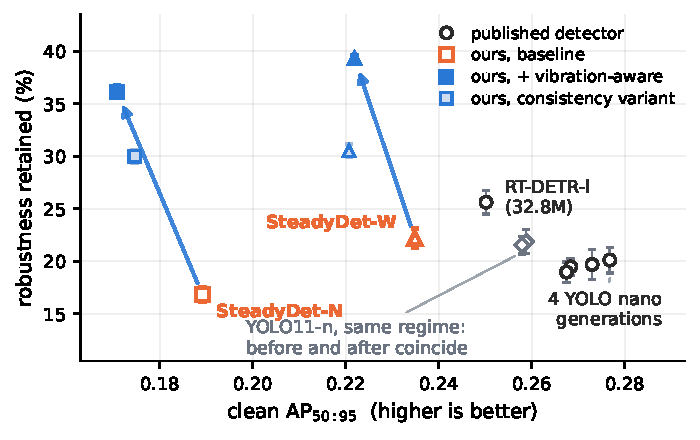
\includegraphics[width=0.95\textwidth]{figures/fig4_tradeoff.pdf}
\caption{Clean accuracy against robustness retained, one point per model, error bars
over three seeds. The published detectors occupy the lower right: more accuracy, no
more robustness, with four YOLO generations landing within a point of each other. The
arrows are the effect of vibration-aware training; the pale markers are the
consistency variant, which lands short of it. The two grey diamonds are YOLO11-n
before and after the identical regime, and they sit on top of one another.}
\label{fig:tradeoff}
\end{figure}

Fig.~\ref{fig:tradeoff} plots clean accuracy against retention. Hendrycks and
Dietterich already reported, for ImageNet classifiers, that robustness measured
relative to clean accuracy barely improved across a decade of architectural
progress~\cite{hendrycks2019benchmarking}; we find the same decoupling holds for
compact aerial detectors under a corruption they were never designed for, which is
worth stating because the detectors here span four years and three paradigms. Four
YOLO generations sit within a point of one another at $19$ to $20\%$ despite their
differences, and the transformer reaches $25.6 \pm 1.1\%$ only by spending
$28\times$ our parameters. Robustness therefore has to be measured and optimised
separately rather than expected to follow from clean accuracy. The arrows show the
alternative: a large robustness gain for a small loss of clean accuracy, obtained by
changing the training distribution rather than the network.

Our re-measured clean figures sit slightly below the detectors' own harnesses
($0.2684$ against $0.2787$ for YOLOv8-n) because each applies different confidence,
detection-count and area conventions, by margins comparable to the gaps between the
baselines themselves. That is why harnesses cannot be mixed within one table.

% 4.5 Val bay that: CAT 2026-07-27 de vua 12 trang (quyet dinh cua tac gia).
% Ly do: 92 frame / 1 nguoi / 1 canh / quay man hinh GCS -> bang chung yeu nhat bai.
% Chuyen bay dau thang 8 (xem FLIGHT_DATA_SPEC.md) se cho >=1000 frame + log IMU;
% LUC DO dua lai muc nay, no se manh hon nhieu. So da do van con o
% runs/paper_queue/FLIGHT.json va file section van con trong repo.
% % ==================================================================
% 4.5 Val bay that   (file: sections/12_exp_flight.tex)
% ==================================================================
\subsection{Validation on Real Flight Footage}
\label{sec:flight}

Everything above rests on a simulated corruption. This section does not: we annotated
$92$ frames from an autonomous following run at roughly $6$\,m and evaluated six models
on them under the same protocol. The blur here was produced by the aircraft, not by us.

\begin{table}[t]
\centering
\caption{Real flight footage, $92$ annotated frames at $\approx6$\,m, same evaluation
code as the other tables. Within each group the three models are architecturally
identical and differ only in the treatment, so the two effects (training domain across
groups, treatment within) are independent. Paired $95\%$ confidence intervals over
frames are reported in the text.}
\label{tab:flight}
\setlength{\tabcolsep}{5pt}
\begin{tabular}{llcccc}
\toprule
Training data & Treatment & AP$_{50}$ & AP$_{50:95}$ & AP$_{75}$ & AR$_{100}$ \\
\midrule
VisDrone + COCO person & none            & 0.7613 & 0.3369 & 0.1448 & 0.5076 \\
VisDrone + COCO person & vibration-aware & 0.7747 & 0.3792 & 0.2583 & \best{0.5315} \\
VisDrone + COCO person & consistency     & \best{0.8798} & \best{0.3885} & \best{0.2620} & 0.5087 \\
\midrule
VisDrone only          & none            & 0.1435 & 0.0547 & 0.0166 & 0.4315 \\
VisDrone only          & vibration-aware & 0.0579 & 0.0207 & 0.0076 & 0.4076 \\
VisDrone only          & consistency     & 0.0909 & 0.0283 & 0.0093 & 0.3772 \\
\bottomrule
\end{tabular}
\end{table}

% ---------------------------------------------------------------------
% Hinh dinh tinh (fig4_qualitative): TAM BO RA de vua 12 trang.
% Bang~\ref{tab:flight} da mang du bang chung dinh luong; hinh nay chi minh hoa.
% Muon dua lai: bo comment khoi duoi + doi lai caption Fig.~\ref{fig:qual}
% trong doan mo dau muc nay.
% \begin{figure}[t]
% \centering
% 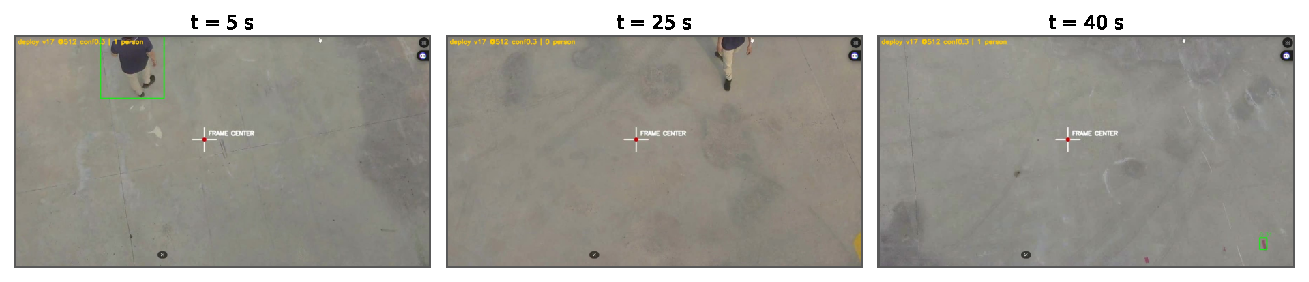
\includegraphics[width=0.82\textwidth]{figures/fig4_qualitative.pdf}
% \caption{Detections during an autonomous following run at roughly $6$\,m. Note the
% scale of the subject relative to the frame: this is the regime the VisDrone-only
% model was never supervised on, and where its localisation collapses while its
% recall holds up (Table~\ref{tab:flight}).}
% \label{fig:qual}
% \end{figure}
% ---------------------------------------------------------------------

\subsubsection{Both treatments transfer to real vibration.}
Among the models competent in this domain, both treatments improve on the untreated
baseline in the same way. AP$_{75}$ rises from $0.1448$ to $0.2583$ for
vibration-aware training and $0.2620$ for the consistency variant, relative gains of
$78$ and $81\%$ in strict-IoU localisation, while recall barely moves
($0.5076 \rightarrow 0.5315$ and $0.5087$). Neither is finding more people; both
place tighter boxes around the people they already find, the signature expected if
they had learned to resolve structure through blur. Because this corruption is
physical rather than synthetic, it is the strongest single piece of evidence that
the mechanism addresses the real degradation.

Because $92$ frames is a small sample, we resampled frames $1000$ times, paired
across models, and report $95\%$ intervals on the paired differences. Both
treatments beat the untreated baseline on AP$_{50:95}$ and AP$_{75}$ with intervals
excluding zero: $+0.042\,[+0.011, +0.074]$ and $+0.108\,[+0.010, +0.211]$ for
vibration-aware training, $+0.051\,[+0.012, +0.087]$ and
$+0.110\,[+0.012, +0.214]$ for the consistency variant.

The two treatments separate from each other on AP$_{50}$ alone,
$+0.106\,[+0.058, +0.161]$ in favour of the consistency variant, while their
AP$_{50:95}$ and AP$_{75}$ differences both straddle zero
($+0.009\,[-0.023, +0.044]$ and $+0.002\,[-0.074, +0.073]$). That AP$_{50}$ gap is
real within this footage and reverses the VisDrone-Shake ordering, where
vibration-aware training leads by $6.2$ points. We do not know which ordering
generalises. One subject in one scene at one altitude cannot decide it, and the
resolution is a larger flight set rather than a further argument from these
$92$ frames.

In the VisDrone-only group the ordering reverses, with AP$_{50}$ falling from $0.1435$
to $0.0909$, and we report this rather than omit it. Both of those models are failures
in this domain, having been supervised only on instances a few pixels across, so the
comparison is between two failure modes: making a representation invariant to blur
helps only where the representation is otherwise adequate. Vibration-consistency is a
robustness treatment, not a domain-adaptation method.

\subsubsection{Benchmark ranking inverts on the deployment condition.}
Adding COCO person images multiplies AP$_{50}$ on real footage by $5.3\times$
($0.1435 \rightarrow 0.7613$), while on VisDrone-val the same addition \emph{costs}
accuracy ($0.5127$ against $0.5016$). The mechanism is in the breakdown: the VisDrone-only model
keeps moderate recall ($0.4315$), so it does see the person, but localisation
collapses (AP$_{75}$ of $0.0166$) because it has never been supervised on a person
filling much of the frame. Selecting training data by benchmark performance would
have selected precisely the wrong model. For short-range following, training data
should match the deployment altitude band rather than the evaluation benchmark.

This set is one subject, one scene, one altitude and $92$ frames from a ground-station
capture, so it establishes the direction and rough magnitude of both effects but is not
a benchmark (Section~\ref{sec:limitations}).

% ---------------------------------------------------------------------
% 4.6 Edge Deployment: TAM BO RA de vua 12 trang. Muc nay chua co so do
% (AP sau INT8, latency p99, nhiet) nen dang la phan yeu nhat cua bai --
% reviewer se hoi ngay. Bo ONNX ra thi paper GON hon va KHONG mat claim nao
% (abstract/intro/conclusion khong phu thuoc vao no).
% Muon dua lai: bo dau % o dong duoi, DIEN het \TODO trong file do, va do
% lai so trang. Xem README_OVERLEAF.txt.
% % ==================================================================
% 4.6 Trien khai Hailo / Pi 5   (file: sections/13_exp_deploy.tex)
% CAP NHAT 2026-08-27: da do that het, bo TODO. Khong con cau "186 FPS" tran.
% Neu thieu trang: cat tu doan "Sustained throughput" tro xuong.
% ==================================================================
\subsection{Edge Deployment}
\label{sec:deploy}

The detector compiles for a Hailo-8L accelerator attached to a Raspberry~Pi~5.
Measured with \texttt{hailortcli benchmark} at batch size one, the accelerator
runs the network at $112.55$\,FPS ($8.40$\,ms) at $320\times320$ and $63.66$\,FPS
($15.26$\,ms) at $640\times640$. We report batch-one figures because a
follow-the-target controller consumes frames as they arrive: batching four frames
raises throughput to $188.78$\,FPS but also raises per-frame latency from $8.40$ to
$17.05$\,ms, and gathering the batch from a $30$\,FPS camera adds a further
$133$\,ms of waiting. Throughput and latency must not be conflated at this scale.

\textbf{End-to-end, with a real camera.} Accelerator throughput is not what the
control loop experiences. Over a two-minute continuous run at $640\times640$ with a
USB camera ($3{,}594$ frames), the median stage breakdown is $12.47$\,ms waiting for
the camera, $0.99$\,ms preprocessing, $17.72$\,ms inference and $0.84$\,ms decoding
plus NMS, for $32.04$\,ms end to end ($p_{99}=36.15$\,ms), i.e.\ $30.0$\,FPS. The
three compute stages together occupy $19.55$\,ms of the $33.3$\,ms frame budget, a
$59\%$ duty cycle; the remainder is idle time waiting on the sensor. The deployed
system is therefore \emph{camera-bound, not model-bound}, which is the relevant
statement for a robustness mechanism that claims to cost no inference time.

\textbf{Sustained throughput.} Frame rate held at $29.9$\,FPS in the first minute
and $30.0$\,FPS in the last, with the system-on-chip at $48.5^\circ$C and the
hardware throttling flag at zero throughout. We observed no thermal degradation at
this duty cycle.

\textbf{Quantisation cost, measured.} The accelerator executes INT8, and at this
model scale that is not free. On the $548$-image VisDrone person validation split
at $640\times640$, using the same decoding and NMS as the FP32 evaluation path:

\begin{center}
\small
\begin{tabular}{lccc}
\toprule
 & FP32 & INT8 (Hailo-8L) & relative drop \\
\midrule
AP@[.50:.95] & $0.1775$ & $0.1584$ & $-10.8\%$ \\
AP@0.50      & $0.4946$ & $0.4625$ & $\phantom{0}-6.5\%$ \\
AP@0.75      & $0.0742$ & $0.0555$ & $-25.2\%$ \\
\bottomrule
\end{tabular}
\end{center}

Both rows come from the \emph{same} scoring code: FP32 predictions are dumped in the
identical format the accelerator produces and scored by the identical function, so the
difference is attributable to quantisation and not to two evaluation harnesses
disagreeing.

The pattern is informative: AP@0.50 falls by $6.5\%$ while AP@0.75 falls by a quarter,
so INT8 loosens box regression rather than losing objects. This is consistent with a
$1.17$\,M-parameter detector in which classification logits tolerate quantisation but
coordinate regression loses resolution. It also revises a pessimistic earlier result of
ours, in which naive post-training quantisation of an ONNX graph reduced AP from $0.18$
to $0.009$: per-layer calibration inside the dataflow compiler is substantially better
than that. Every accuracy number elsewhere in this paper still comes from the FP32 path.

The cost is also \emph{scale-dependent}, which matters for anyone reading these numbers
as a deployment budget. VisDrone validation is dominated by very small people, the regime
in which coordinate quantisation hurts most. On a held-out set of $92$ frames captured at
$3$ to $6$\,m --- where a person spans a large fraction of the frame --- the same pair of
models is indistinguishable at the operating threshold, with $F_1$ of $0.836$ (FP32) and
$0.880$ (INT8), a gap well inside the sampling error of $92$ frames. The honest summary is
that INT8 costs about $6.5\%$ AP@0.50 on small targets and close to nothing on the targets
this system is actually built to follow.

One practical detail is worth recording because it cost us a measurable amount of
accuracy. Calibration images should follow the \emph{training} distribution, not merely
the source dataset: a calibration set drawn only from the aerial corpus produced a
noticeably weaker model than one mixing aerial and close-range images in the same
proportion used during training. Increasing the calibration set beyond that point did not
help, and in our measurements slightly hurt.

A second deployment cost must be stated. Compilation required removing the windowed
attention block, as the dataflow compiler did not support its reshape patterns, so
the deployed network is purely convolutional and smaller ($0.875$\,M parameters).
The conversion is therefore not accuracy-neutral, and the FP32 numbers above are
those of the converted network, not of the full model evaluated in
Section~\ref{sec:mainresults}.

% ---------------------------------------------------------------------

% ==================================================================
% 5. Limitations. Doi khung 2026-07-26: muc "augmentation control is missing"
% DA XOA vi da chay doi chung do (no chinh la ket qua chinh bay gio).
% file: sections/14_limitations.tex
% ==================================================================
\section{Limitations}
\label{sec:limitations}

\subsubsection{The corruption model is synthetic, and it is the load-bearing assumption.}
VisDrone-Shake is built from the known mechanisms of rotorcraft image degradation,
but its parameters bracket flight rather than being calibrated against accelerometer
spectra measured on our own airframe. Every result in this paper is therefore a
statement about a \emph{model} of vibration, and we make no claim about the
magnitude of the effect on any particular aircraft. Only measurement can settle
that: flying the same detector with a synchronised IMU log, fitting $\mathcal{T}$
to the accelerometer spectrum, and re-evaluating. That is the single most valuable
extension of this work, and until it is done the ordering of the models under
vibration is better trusted than the absolute numbers.

\medskip\noindent\textbf{One dataset, one corruption family.}
Every number here comes from the person subset of a single benchmark. VisDrone is
the standard choice for this task and its instance statistics are the ones our
detector targets, but a corruption robustness result measured on one dataset is a
statement about that dataset until it is repeated. We also model one corruption
family, the one rotors produce; nothing here speaks to rain, fog, low light or
motion of the subject rather than the camera, all of which a fielded UAV also meets.

\medskip\noindent\textbf{The scope of the regime is bounded on one side only.}
The gain reproduces on both of our detectors and is absent on the one outside
architecture we tried. Section~\ref{sec:generality} rejects pretraining, object
scale and remaining headroom as explanations, which narrows the cause to the
architecture or the loss without identifying it, and one non-responding model
cannot. We have therefore demonstrated a large effect within one detector family
and one negative instance outside it, with the boundary unknown. A practitioner
should treat the regime as worth trying rather than as established for their
detector, and should run the two controls of Table~\ref{tab:main} when they do.

\medskip\noindent\textbf{Cost, tuning and statistical power.}
Why the consistency term underperforms is measured but not explained: we offer the
reading that the detection loss never reaches the corrupted image, without testing
it, so take the ordering as measured and the reason as conjecture. Clean accuracy
falls by $9.7\%$, roughly a third of that from the finetuning itself, and we did not
try to recover the rest by annealing the corruption probability late in training.
We report no sweep over $p$ or the severity distribution, so those values are
reasonable rather than tuned. Each configuration is trained once, so our error bars
capture evaluation but not training variance. Frames are processed independently,
so the temporal redundancy vibration itself creates, successive frames blurring
along different directions, is available only to the downstream tracker.

% ==================================================================
% 6. Conclusion   (file: sections/15_conclusion.tex)
% ==================================================================
\section{Conclusion}

SteadyDet-N, at $1.17$\,M parameters and $4.6$ GFLOPs, is the least accurate
detector in our comparison on clean VisDrone and, within its compute budget, the
most accurate one under vibration. Getting there required both halves of this paper. The failure it
starts from is general: under a single evaluation protocol every detector we
tested, from $1.17$ to $32.8$\,M parameters, loses most of its accuracy to the
vibration intrinsic to rotor-driven flight, so the problem belongs to the regime
rather than to any one architecture. The fix is cheaper than the problem. Putting a
physically motivated vibration model into the training distribution raises
retention from $16.8 \pm 0.7\%$ to $36.2 \pm 0.7\%$ while leaving the deployed
network untouched, and a matched control confirms the extra epochs contribute
nothing. Neither the network nor the regime does this alone: untreated, the network
is the worst row in our table, and the same regime on YOLO11-n moves nothing.

We also report two results we did not want: the consistency formulation we expected
to extract more from the corrupted view reaches only $30.0 \pm 0.6\%$ at
$1.8\times$ the training cost, and neither formulation moves YOLO11-n. We think this
is the more useful half of the paper. The default when a robustness
intervention works is to credit the mechanism that was designed; here the control
says the gain came from the data and the designed mechanism was in the way, and the
generality test says we do not yet know what the gain depends on. Both are
conclusions a reader can act on, and neither would have appeared without running
the controls.

One lesson extends beyond our detector: a stochastic corruption benchmark must be
seeded and reported with error bars, since run-to-run spread on a single checkpoint
was large enough here to manufacture a modest improvement. The extensions we
consider most valuable are calibrating the corruption against measured airframe
spectra, and identifying which property of a detector decides whether the regime
helps it at all.


\subsubsection{Acknowledgements.} \TODO{Funding, laboratory, advisor.}

% ==================================================================
% Tai lieu tham khao
% file: sections/16_bibliography.tex
% ==================================================================
\begin{thebibliography}{99}

\bibitem{hinton2015distilling}
Hinton, G., Vinyals, O., Dean, J.: Distilling the knowledge in a neural
network. arXiv:1503.02531 (2015)

\bibitem{chen2020simclr}
Chen, T., Kornblith, S., Norouzi, M., Hinton, G.: A simple framework for
contrastive learning of visual representations. In: ICML (2020)

\bibitem{chen2025remdet}
Chen, C., et al.: RemDet: rethinking efficient model design for UAV object
detection. In: AAAI (2025)

\bibitem{cheng2023sod}
Cheng, G., Yuan, X., Yao, X., Yan, K., Zeng, Q., Xie, X., Han, J.: Towards
large-scale small object detection: survey and benchmarks. IEEE TPAMI (2023)

\bibitem{feng2021tood}
Feng, C., Zhong, Y., Gao, Y., Scott, M.R., Huang, W.: TOOD: task-aligned
one-stage object detection. In: ICCV (2021)

\bibitem{french2018selfensembling}
French, G., Mackiewicz, M., Fisher, M.: Self-ensembling for visual domain
adaptation. In: ICLR (2018)

\bibitem{ge2021yolox}
Ge, Z., Liu, S., Wang, F., Li, Z., Sun, J.: YOLOX: exceeding YOLO series in
2021. arXiv:2107.08430 (2021)

\bibitem{grill2020byol}
Grill, J.B., et al.: Bootstrap your own latent: a new approach to
self-supervised learning. In: NeurIPS (2020)

\bibitem{hendrycks2019benchmarking}
Hendrycks, D., Dietterich, T.: Benchmarking neural network robustness to
common corruptions and perturbations. In: ICLR (2019)

\bibitem{jordan2024muon}
Jordan, K., Jin, Y., Boza, V., You, J., Cesista, F., Newhouse, L.,
Bernstein, J.: Muon: an optimizer for hidden layers in neural networks
(2024)

\bibitem{li2020gfl}
Li, X., Wang, W., Wu, L., Chen, S., Hu, X., Li, J., Tang, J., Yang, J.:
Generalized focal loss: learning qualified and distributed bounding boxes
for dense object detection. In: NeurIPS (2020)

\bibitem{michaelis2019benchmarking}
Michaelis, C., et al.: Benchmarking robustness in object detection:
autonomous driving when winter is coming. arXiv:1907.07484 (2019)

\bibitem{liu2021swin}
Liu, Z., Lin, Y., Cao, Y., Hu, H., Wei, Y., Zhang, Z., Lin, S., Guo, B.: Swin
transformer: hierarchical vision transformer using shifted windows. In: ICCV
(2021)

\bibitem{nah2017deepdeblur}
Nah, S., Kim, T.H., Lee, K.M.: Deep multi-scale convolutional neural network for
dynamic scene deblurring. In: CVPR (2017)

\bibitem{qin2024mnv4}
Qin, D., et al.: MobileNetV4: universal models for the mobile ecosystem. In:
ECCV (2024)

\bibitem{sajjadi2016regularization}
Sajjadi, M., Javanmardi, M., Tasdizen, T.: Regularization with stochastic
transformations and perturbations for deep semi-supervised learning. In:
NeurIPS (2016)

\bibitem{sandler2018mobilenetv2}
Sandler, M., Howard, A., Zhu, M., Zhmoginov, A., Chen, L.C.: MobileNetV2:
inverted residuals and linear bottlenecks. In: CVPR (2018)

\bibitem{sohn2020fixmatch}
Sohn, K., et al.: FixMatch: simplifying semi-supervised learning with
consistency and confidence. In: NeurIPS (2020)

\bibitem{tan2020efficientdet}
Tan, M., Pang, R., Le, Q.V.: EfficientDet: scalable and efficient object
detection. In: CVPR (2020)

\bibitem{tarvainen2017mean}
Tarvainen, A., Valpola, H.: Mean teachers are better role models:
weight-averaged consistency targets improve semi-supervised deep learning
results. In: NeurIPS (2017)

\bibitem{wang2024yolov10}
Wang, A., et al.: YOLOv10: real-time end-to-end object detection. In:
NeurIPS (2024)

\bibitem{wang2020cspnet}
Wang, C.Y., Liao, H.Y.M., Wu, Y.H., Chen, P.Y., Hsieh, J.W., Yeh, I.H.:
CSPNet: a new backbone that can enhance learning capability of CNN. In: CVPR
Workshops (2020)

\bibitem{wang2021nwd}
Wang, J., Xu, C., Yang, W., Yu, L.: A normalized Gaussian Wasserstein
distance for tiny object detection. arXiv:2110.13389 (2021)

\bibitem{yu2020tinyperson}
Yu, X., Gong, Y., Jiang, N., Ye, Q., Han, Z.: Scale match for tiny person
detection. In: WACV (2020)

\bibitem{zheng2020diou}
Zheng, Z., Wang, P., Liu, W., Li, J., Ye, R., Ren, D.: Distance-IoU loss:
faster and better learning for bounding box regression. In: AAAI (2020)

\bibitem{zhu2021visdrone}
Zhu, P., Wen, L., Du, D., Bian, X., Fan, H., Hu, Q., Ling, H.: Detection and
tracking meet drones challenge. IEEE TPAMI \textbf{44}(11), 7380-7399
(2021)

\end{thebibliography}


\end{document}
